\documentclass{minimal}
\usepackage{microtype}
\DisableLigatures{encoding=*,family=*}
\usepackage{tikz}
\usetikzlibrary{backgrounds,decorations.pathmorphing,arrows.meta,positioning}

\begin{document}
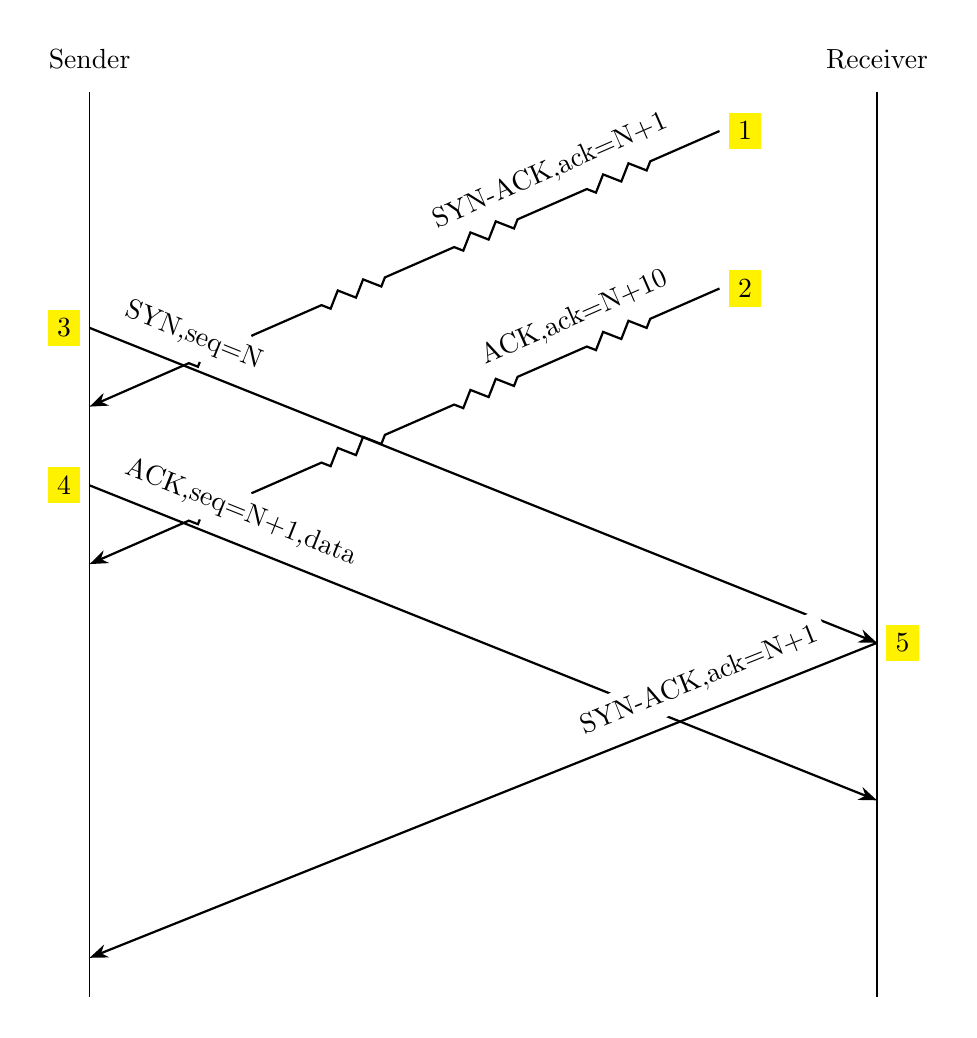
\begin{tikzpicture}
  [
    show background rectangle,
    background rectangle/.style = {fill=white},
    endpoint/.style = {above,yshift=5},
    packet line/.style = thick,
    delayed/.style = {decorate,decoration=straight zigzag},
    send id/.style = {left,xshift=-3,fill=yellow},
    recv id/.style = {right,xshift=3,fill=yellow},
    send info/.style = {pos=0.02,above,sloped,anchor=south west,fill=white,yshift=3},
    recv info/.style = {pos=0.05,above,sloped,anchor=south east,fill=white,yshift=3},
    > = Stealth,
  ]

  \draw (0,1)  node[endpoint] {Sender}   -- (0,-10.5);
  \draw (10,1) node[endpoint] {Receiver} -- (10,-10.5);

  \draw [->, packet line, delayed] (8,0.5)  node[recv id] {1} -- node[recv info] {SYN-ACK,ack=N+1}  (0,-3);
  \draw [->, packet line, delayed] (8,-1.5) node[recv id] {2} -- node[recv info] {ACK,ack=N+10}     (0,-5);
  \draw [->, packet line] (0,-2)   node[send id] {3} -- node[send info] {SYN,seq=N}        (10,-6);
  \draw [->, packet line] (0,-4)   node[send id] {4} -- node[send info] {ACK,seq=N+1,data} (10,-8);
  \draw [->, packet line] (10,-6)  node[recv id] {5} -- node[recv info] {SYN-ACK,ack=N+1}  (0,-10);

\end{tikzpicture}
\end{document}
